\chapter{Analiza problemu}
\thispagestyle{chapterBeginStyle}
\label{rozdzial1}

W tym rozdziale została przedstawiona analiza zagadnienia. Nakreślono problemy i omówiono proponowane przez system rozwiązania. Omówiono założenia funkcjonalne i niefunkcjonalne samego systemu jak i jego podsystemów.


\section{Charakterystyka problemu}
Aplikacje webowe, a w szczególności systemy e-commerce, są często wolne. Pisane przez niedoświadczonych deweloperów pod presją czasu nie zawsze wychodzą tak jak powinny. Więc jak powinny być napisane? W pierwszej kolejności muszą być dobrze przemyślane, a co za tym idzie ich architektura powinna być przygotowana na rozszerzenia i modyfikacje. Powiedzmy, że mamy sklep internetowy, na bazie którego chcielibyśmy stworzyć jakiś inny sklep. Często jest to niemożliwe ze względu na budowę i obsługę komponentów. Dobrym przykładem na to jest indeksowanie produktów do mechanizmu wyszukującego.
\begin{example}
	W systemie istnieje klasa Product z zadeklarowanymi polami biznesowymi, powiedzmy że klient chce nowe pole o nazwie myCustomField, oczywiście ma być ono wyszukiwalne. Rozszerzamy więc klasę Produkt do MyProdukt i dodajemy pole myCustomField. Mechanizm indeksacji nie ma możliwości wyciągnąć z Produktu pola dotyczącego klasy MyProdukt, ponieważ zaprzeczałoby to zasadom polimorfizmu.
\end{example} 
To tylko konkretny przykład, ale warto zwrócić uwagę, że dotyczy on nie tylko produktów, a i również jakichkolwiek encji, którymi chcemy zarządzać w systemie. To pierwszy problem rozwiązań e-commerce, które nie są oparte o elastyczne frameworki. 

Kolejną rzeczą idącą za słabą architekturą są tak zwane bottlenecki\footnote{bottleneck - wspólny punkt dla aplikacji, przez muszą przejść użytkowicy korzystając z różnych funkcjonalności}, które blokują szybkie działanie aplikacji. Przykład z życia: 
\begin{example}
	Nasza platforma jest oparta o framework stworzony parę lat temu, do tego taki, który nie jest open-source, ma architekturę monolityczną. Nasz sklep zyskał na popularności i coraz częściej zdarzają nam się awarię związane z ograniczoną wydajnością, najszybszą i naturalną reakcją jest dokupienie nowego serwera do obsługi większej ilości klientów, jednak wiąże się to z bardzo dużymi kosztami.
\end{example} 
W tym przykładzie warto zwrócić uwagę na zamknięty charakter frameworku. Brak licencji open-source często skutkuje to tym, że projekt jest skazany na zamknięty cykl rozwoju (o ile w ogóle jest dalej rozwijany), ewentualne błędy nie mogą być naprawione \textit{od ręki}. Raz napisana platforma komercyjna nie będzie po 5 latach wcale aktualna. Inaczej sprawy się mają w przypadku open-source'wych frameworków, gdzie istnieje możliwość zmiany technologi, a aktualizacje są dostępne praktycznie zawsze. To dzięki zasadzie \textit{inversion of control}, kiedy to programista decyduje się na oddanie kontroli nad częścią swojej funkcjonalności w ręce używanego przez siebie frameworku, aktualizacja do nowszych wersji używanych technologii jest zwykle bezbolesna i opiera się głównie na zmianie wersji w pliku konfiguracyjnym zależności projektowe.

Następny problem związany ze środowiskiem e-commerce to brak dobrych wyszukiwarek produktów na stronach. Często zdarza się, że wyszukiwarki przeszukują relacyjne bazy danych, zamiast korzystać z płaskich struktur jakie oferują nam rozwiązania typu noSQL. Do tego nie obsługują facetów \footnote{wyjaśnienie terminu dostępne w sekcji \textbf{Słowniczek}}, co sprawia trudności z wyszukaniem produktu i dopasowaniem go pod klienta, a przecież to jest główny założenie tego biznesu. Jasne i wiadome jest, że istnieją sklepy z dobrymi wyszukiwarkami, do tego mogące pochwalić się wysokim miernikiem TPS\footnote{\textit{TPS} -- transaction per second, ilość pełnych requestów wraz z odpowiedzią, jaką może obsłużyć serwer na sekundę.}. Jednakże są to rozwiązania bardzo drogie i niedostępne dla małych przedsiębiorstw. Z drugiej strony implementowanie takich funkcjonalności na własną rękę jest również bardzo drogie, a do tego skomplikowane. W tym momencie z pomocą przychodzą właśnie darmowe frameworki, jednak nie wszystkie maja pełna obsługe mechanizmu indeksującego.

Istotną sprawą w opisywanych systemach jest archiwizacja produktu, bądź jej zupełny brak. Problem został opisany na poniższym przykładzie:
\begin{example}
	Klient zakupił produkt A o atrybutach (a, b, c, d) w sierpniu. W październiku manager sklepu zmienił atrybuty produktu A na (e, f, g), co wpłynęło również na cenę. W listopadzie klient zdecydował się na reklamację produktu. Obsługa sklepu otrzymała zgłoszenie, ma id produktu, jednak niewiele to pomoże, gdyż atrybuty i cena uległy zmianie. 
\end{example}

Ostatnią, nie mniej jednak ważną rzeczą, która warta jest opisania to sposób, w jaki charakteryzuje się produkty\footnote{ lub cokolwiek innego podlegającego klasyfikacji} w sklepach internetowych. Produkty należy opisywać w konsekwentny i najbardziej jednoznaczny sposób, jednak nie da się tego osiągnąć bazując tylko na polach ewentualnej klasy Produkt, ponieważ jest to wybitnie nieelastyczne, każda zmiana wymaga wtedy trwałej ingerencji w kod i ponowny release.

Powyższe problemy niektórych systemów e-commerce można sprowadzić do następujących stwierdzeń:
\begin{itemize}
	\item architektura nieprzygotowana pod nagłe modyfikacje i rozszerzenia
	\item najczęściej używane punkty aplikacji nie są odseparowane od reszty
	\item brak dobrych wyszukiwarek i mechanizmów filtrujących
	\item niekonkretny i mało abstrakcyjny sposób opisu encji biznesowych
	\item użycie zamkniętych technologi, nie korzystanie z open-source, brak zastosowania \textit{inversion of control}
	\item brak archiwizacji produktów
\end{itemize}

\section{Proponowane rozwiązania - wymagania funkcjonalne}
Jasno zdefiniowane problemy same nasuwają pewne rozwiązania, dlatego poniżej określono listę następujących wymagań funkcjonalnych:
\begin{itemize}
	\item wykorzystanie najnowszych technologii oraz IoC
	\item podłączony zewnętrzny serwer Apache Solr, służący do bardzo szybkiej obsługi zapytań związanych z katalogiem produktowym,
	\item prosty i efektywny system klasyfikacyjny dla produktów,
	\item reużywalny i rozszerzalny panel administracyjny 
	\item zaawansowana obsługą uprawnień dla panelu administracyjnego,
	\item elastyczny model, pozwalający na rozszerzanie klas bez konieczności ingerowania w strukture systemu
	\item łatwy w skonfigurowaniu i wydajny mechanizm wyszukiwania,
	\item relacyjna i nierelacyjna baza danych,
	\item zaiplementowana obsługa procesu zamówienia,
	\item mechanizm wersjonowania produktu.
\end{itemize} 

Rysunek \ref{wymagania} ilustruje pokrycie znalezionych problemów wymaganiami funkcjonalnymi opisywanego frameworka. Wynika z niego, że \textit{bez pokrycia} zostają dwa wymagania, nie oznacza to jednak, że są to niepotrzebne funkcjonalności. Są jednak powszechnie spotykane w frameworkach e-commerce, można nazwać je standardem. Jednak co mniej oczywiste system uprawnień został oparty na strukturze drzewiastej, uprawnienia są dziedziczone pomiędzy użytkownikami finalnego systemu opartego o framework.
\begin{figure}
	\begin{center}
		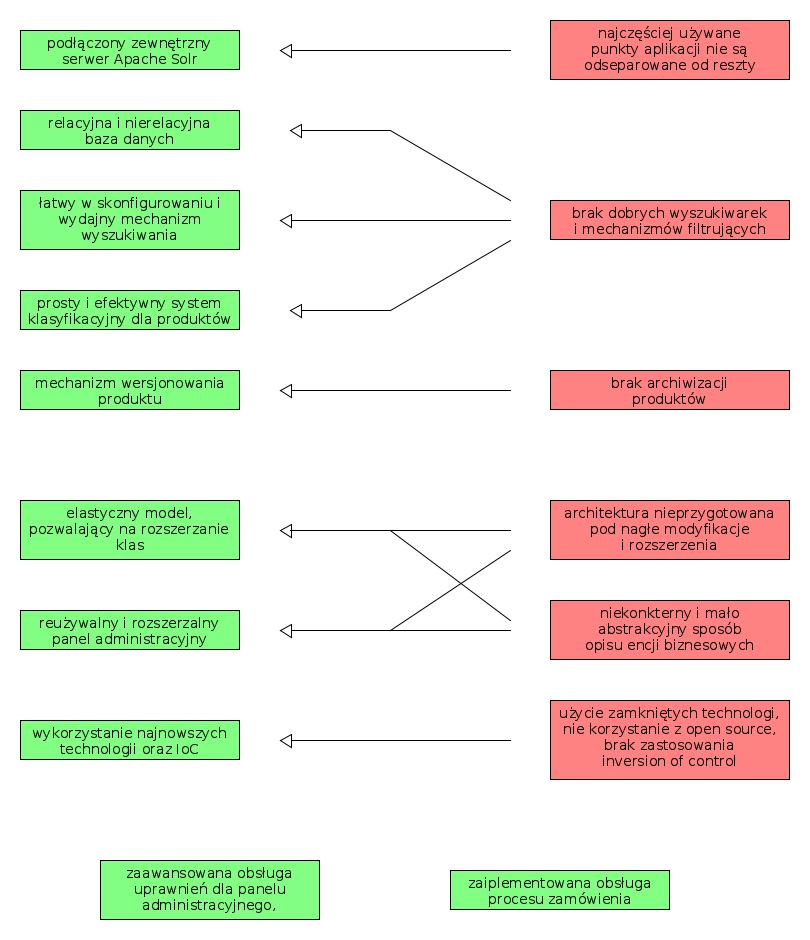
\includegraphics[width=1\textwidth]{wymagania.jpg}
	\end{center}
	\caption{{\color{dgray}Połączenie wymagań funkcjonalnych ze znalezionymi problemami.}} \label{wymagania}
\end{figure}
